
%(BEGIN_QUESTION)
% Copyright 2008, Tony R. Kuphaldt, released under the Creative Commons Attribution License (v 1.0)
% This means you may do almost anything with this work of mine, so long as you give me proper credit

Denne nivåreguleringsventilen kaviterer når vann strømmer gjennom den. En trykkprofilgraf viser ventilens innløpstrykk ($P_1$), utløpstrykk ($P_2$) og vena contracta-trykk ($P_{vc}$), lagt over en stiplet linje som viser vannets damptrykk:

$$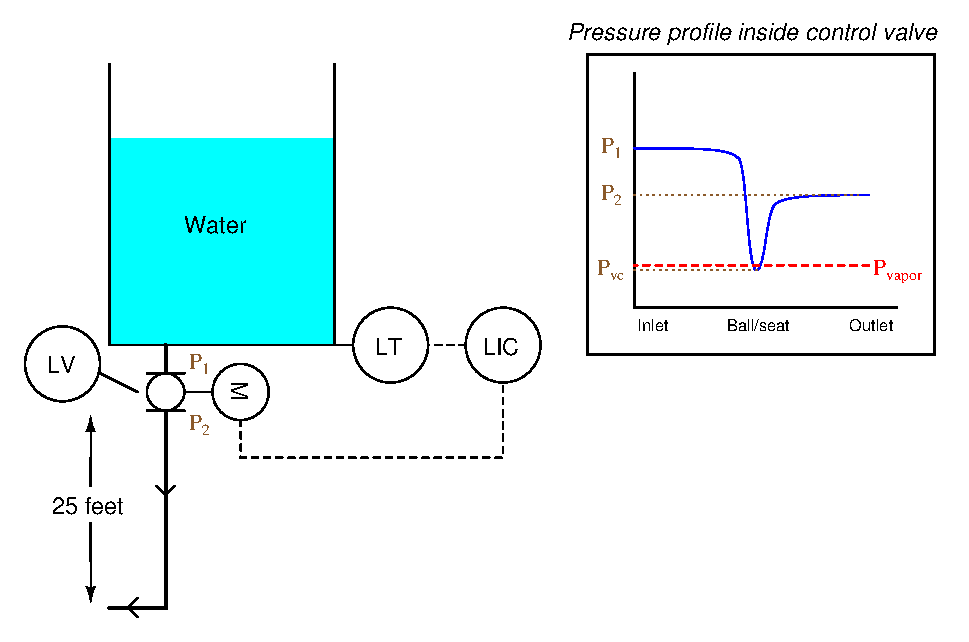
\includegraphics[width=15.5cm]{i01419x01.eps}$$

Forklar hvorfor denne ventilen kaviterer, og inkluder data fra ventilens trykkprofil i forklaringen.

\vskip 10pt

\filbreak

Senere bestemmer en prosessingeniør seg for å flytte den samme reguleringsventilen til en lavere posisjon på røret. Nå kaviterer ikke ventilen lenger, selv med nøyaktig samme strømningsrate gjennom ventilen ($Q$) og samme trykkfall ($P_1 - P_2$)! En ny trykkprofilgraf viser hvordan alle trykk i alle punkter inne i reguleringsventilen har endret seg som resultat av flyttingen:

$$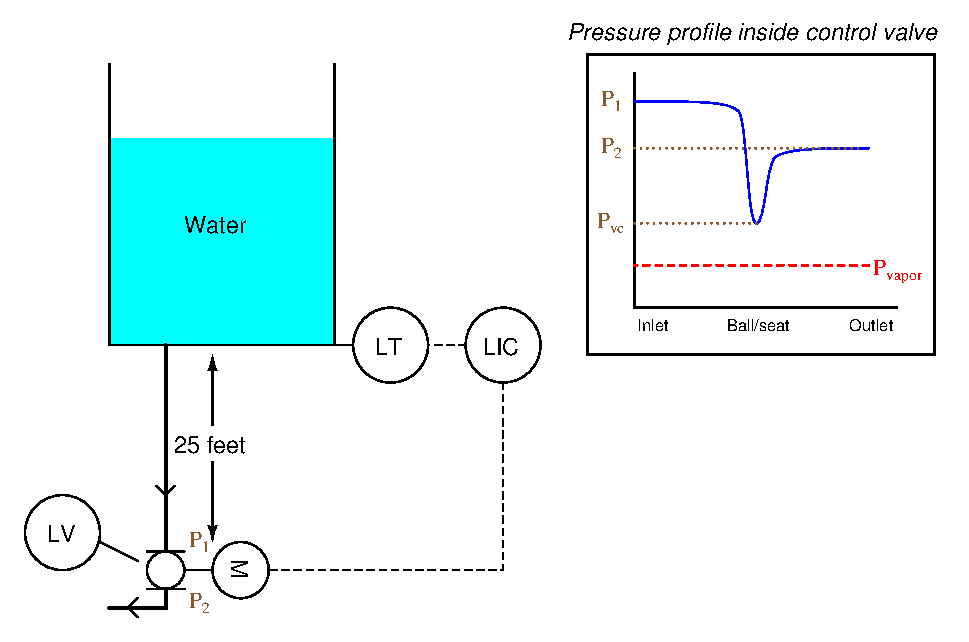
\includegraphics[width=15.5cm]{i01419x02.eps}$$

Forklar hvorfor ingeniørens løsning virket, og inkluder data fra den endrede trykkprofilen i forklaringen. Oppgi også minst én {\it annen} endring som kunne vært gjort i prosessen for å redusere eller eliminere kavitasjon, utover å flytte ventilen.

\vskip 20pt \vbox{\hrule \hbox{\strut \vrule{} {\bf Forslag til sokratisk diskusjon} \vrule} \hrule}

\begin{itemize}
\item{} Forklar hva begrepet ``damptrykk'' betyr for et stoff
\item{} Ville ingeniørens løsning fungert dersom vannet strømmet {\it motsatt} vei gjennom ventilen (altså {\it opp} inn i beholderen i stedet for {\it ned} ut av beholderen)? Hvorfor eller hvorfor ikke?
\item{} Hvilken type reguleringsventil og aktuator brukes i denne applikasjonen?
\end{itemize}

\underbar{file i01419}
%(END_QUESTION)





%(BEGIN_ANSWER)

Ny ventilplassering øker absolutt trykk i alle punkter inne i ventilen, slik at det laveste trykket ($P_{vc}$) aldri faller under vannets damptrykk. Jeg lar deg identifisere andre løsninger.
 
%(END_ANSWER)





%(BEGIN_NOTES)

Andre løsninger:

\begin{itemize}
\item{} Bytt til en type reguleringsventil med større trykkgjenvinningsfaktor ($F_L$), som er det samme som å si en ventil med {\it mindre} trykkgjenvinning.
\vskip 5pt
\item{} Installer en annen reguleringsventil med trim for ``kavitasjonskontroll''
\vskip 5pt
\item{} Senk vanntemperaturen
\end{itemize}

\vskip 10pt

Når ventilen er plassert øverst i et 25 fot vertikalt rørfall, arbeider den ved svært lave statiske trykk på grunn av delvakuumet som oppstår på nedstrømssiden fra den vertikale vannsøylen i røret (-25 fot = -10.84 PSI). Når ventilen plasseres nær bunnen av dette 25 fots rørfallet, havner nivåhøyde-trykket på oppstrømssiden som en positiv størrelse i stedet for en negativ størrelse.

Videre kan det være nødvendig å bytte ventilen til globetype i stedet for kuletype, siden kuleventiler fremmer kavitasjon på grunn av høy trykkgjenvinningsgrad (liten $F_{L}$-faktor).

\vfil \eject

\noindent
{\bf Oppsummeringsquiz:}

Nevn én praktisk måte å enten forhindre eller redusere de skadelige virkningene av kavitasjon i en reguleringsventil, utover å installere en ventil med spesialtrim mot kavitasjon.


%INDEX% Final Control Elements, valve: cavitation control

%(END_NOTES)

